\documentclass[10pt,twocolumn,letterpaper]{article}

\usepackage{cvpr}
\usepackage{times}
\usepackage{epsfig}
\usepackage{graphicx}
\usepackage{amsmath}
\usepackage{amssymb}

% Include other packages here, before hyperref.
\newcommand{\rak}[1]{{\color{orange}{rak: #1}}}
\newcommand{\ma}[1]{{\color{purple}{ma: #1}}}
\newcommand{\mgm}[1]{{\color{cyan}{mgm: #1}}}

% If you comment hyperref and then uncomment it, you should delete
% egpaper.aux before re-running latex.  (Or just hit 'q' on the first latex
% run, let it finish, and you should be clear).
\usepackage[breaklinks=true,bookmarks=false]{hyperref}

\cvprfinalcopy % *** Uncomment this line for the final submission

\def\cvprPaperID{****} % *** Enter the CVPR Paper ID here
\def\httilde{\mbox{\tt\raisebox{-.5ex}{\symbol{126}}}}

% Pages are numbered in submission mode, and unnumbered in camera-ready
%\ifcvprfinal\pagestyle{empty}\fi
\setcounter{page}{4321}
\begin{document}

%%%%%%%%% TITLE
\title{DREU Final Report}

\author{Madeleine Grunde-McLaughlin\\
University of Pennsylvania\\
Philadelphia, Pennsylvania\\
{\tt\small mgrund@sas.upenn.edu}
% For a paper whose authors are all at the same institution,
% omit the following lines up until the closing ``}''.
% Additional authors and addresses can be added with ``\and'',
% just like the second author.
% To save space, use either the email address or home page, not both
\and
Maneesh Agrawala\\
Stanford University\\
Palo Alto\\
{\tt\small maneesh@cs.stanford.edu}
}

\maketitle
%\thispagestyle{empty}

%%%%%%%%% ABSTRACT
%\begin{abstract}
%	Unnecessary for DREU Final?
%\end{abstract}

%%%%%%%%% BODY TEXT
\section{Introduction}

\mgm{Looking into the actual lengths, a lot esp in test set are shorter than 30 seconds. may want to find average}

\mgm{High level comment: is this too much or too little detail for an intro? anything else we should include?}

\mgm{Is this a useful thing to include: Few questions in existing benchmarks focus specifically on object manipulation through videos.} 

The ability to perceive and reason about human activity has been a long standing goal for Computer Vision. Research in Cognitive Science and Neuroscience suggests that humans decompose actions into a hierarchy of parts \cite{zacks2001events}. Therefore, in order to reason about activities, models should be capable of spatial and temporal reasoning over a subject's changing relationships with objects \cite{ji2020action}. One task developed to measure visual reasoning abilities is Visual Question Answering (VQA), in which a model answers questions about a visual input. 

A variety of benchmarks have been created to test a model's abilities at the VQA task. ImageQA benchmarks take images as input \cite{johnson2017clevr, hudson2019gqa, antol2015vqa, zellers2019recognition, goyal2017making, krishna2017visual, zhu2016visual7w, kim2020answering} and VideoQA benchmarks take videos as input \cite{tapaswi2016movieqa, lei2018tvqa, jang2017tgif, kim2017deepstory, xu2017video, maharaj2017dataset, zeng2016leveraging, yu2019activitynet}. Since most VQA benchmarks are image-based, they can test reasoning on spatial relationships, object attributes, and common sense understanding, but they cannot test reasoning over temporal relationships or activities. 

For this reason, a growing number of VideoQA benchmarks have been release, but current benchmarks exhibit some weaknesses. First, many involve short videos ($<$ 10 seconds) \cite{jang2017tgif, kim2017deepstory, xu2017video, maharaj2017dataset}, or contain fewer than 200k questions \mgm{what counts as small?} \cite{tapaswi2016movieqa, lei2018tvqa, kim2017deepstory, xu2017video, jang2017tgif, yu2019activitynet, zeng2016leveraging}. 

Second, current benchmarks require at most two reasoning steps to answer. For example, the question "What happened to the woman before playing violin?" requires first finding when the woman played violin, then looking at what happened before then. \cite{yu2019activitynet}). Existing benchmarks also do not use logical or comparative operators in their questions, which leaves out interesting and relevant ideas (e.g. "Which activity did they do for longer?"). Leaving out questions that require more varied reasoning steps creates weaker benchmarks since many VideoQA models get stuck when faced with questions that require multiple reasoning steps \cite{fan2019heterogeneous}. 

Third, several of these benchmarks integrate visual cues with dialogue and plot summaries \cite{lei2018tvqa, tapaswi2016movieqa, kim2017deepstory}. Their analysis found that question answering models depend more heavily on the dialogue input than on the visual input, reducing these benchmarks' effectiveness at measuring visual temporal reasoning \cite{tapaswi2016movieqa, lei2018tvqa}. 

Fourth, after the release of the first large ImageQA datasets, investigations found that their answer distributions were heavily skewed. This bias towards very common answers effectively reduces dependence on visual input and inflates accuracy scores \cite{goyal2017making, hudson2019gqa}. Some ImageQA datasets have worked to balance answer distributions, but to our knowledge no VideoQA datasets have systematically balanced answer distributions \cite{goyal2017making, hudson2019gqa}. 

Finally, existing benchmarks have accuracy measurements only for the overall dataset and sometimes for each question type (e.g. Repetition Count, Repeating Action, State Transition, and Frame-based questions in \cite{jang2017tgif}). Reasoning about videos requires multi-step reasoning, comparative and counting operators, flexibility with video length, appearance feature understanding, and fine and coarse motion understanding. A wider metrics suite would improve measurement of models' relative strengths and weaknesses across these many categories.

We propose a VideoQA benchmark that addresses these concerns. Our benchmark is automatically generated in a pipeline inspired by \cite{hudson2019gqa} to combine question templates with Charades action annotations and Action Genome's spatio-temporal scene graphs. This process combines a variety of linguistic structures with the content of over \mgm{10,000} videos, producing \mgm{add here} questions. These questions have a wide variety of lengths, complexities, and structures. With this generation pipeline, we have tight control over the contents of each question, allowing us to balance the answer distribution and create a wide suite of metrics.

We have made much progress within the DREU timeline, and we plan to continue the project through the fall. This final report discusses the questions for 500 videos, \mgm{? template and ? question-answer pairs} By the end of our contributions will be: 1) a large VideoQA dataset of question answer pairs requiring multi-step reasoning and 2) a wide suite of metrics to thoroughly evaluate current models.

\section{Prior Work}

\subsection{ImageQA}

At first, the Visual Question Answering task was mostly restricted to ImageQA. A wide variety of benchmarking datasets were created with the hopes of analyzing the reasoning abilities of ImageQA models \cite{johnson2017clevr, hudson2019gqa, antol2015vqa, zellers2019recognition, goyal2017making, krishna2017visual, zhu2016visual7w, kim2020answering}. Benchmarks vary in input, from synthetic datasets \cite{johnson2017clevr}, to cartoons \cite{antol2015vqa}, to charts \cite{kim2017deepstory}, to real-world images \cite{hudson2019gqa, krishna2017visual, zhu2016visual7w, goyal2017making, zellers2019recognition, antol2015vqa}. They also vary in the type of questions asked, from the 7W's (who, what, where, when, which, why, how) \cite{zhu2016visual7w}, to commonsense reasoning \cite{zellers2019recognition}, to compositional reasoning \cite{johnson2017clevr, hudson2019gqa}, to spatial localization \cite{zhu2016visual7w, krishna2017visual, hudson2019gqa}. These benchmarks facilitated the development of many models made to tackle these challenges by measuring their spatial reasoning abilities \cite{johnson2017clevr, hudson2019gqa, krishna2017visual}. 

However, many of these datasets contained real world priors exacerbated by human annotation bias, resulting in inflated accuracy scores and a lack of understanding of the actual reasoning abilities of these models \cite{goyal2017making, hudson2019gqa}. For example, in the VQA1.0 dataset, 41\% of answers  for questions starting with "What sport is..." were "Tennis". These types of priors meant that models could answer over 50\% of the questions correctly without considering the visual input \cite{goyal2017making}. Once these issues came to light, some new benchmarks attempted to mitigate these biases. VQA2.0 took many of the questions from VQA1.0 and added a similar picture leading to a different answer. This procedure helped, but was only applied to 71\% of questions due to annotation difficulties. Models measured on VQA2.0 could still answer 67\% of binary questions and 27\% of open questions correctly without seeing visual input \cite{hudson2019gqa}. The GQA dataset addressed these biases by creating equal numbers of binary yes/no questions per category, and smoothing the answer distribution in open ended questions. This balancing of the answer distribution retains but reduces the power of real world priors \cite{hudson2019gqa}. Our benchmark is similar to GQA in that it mitigates biases by smoothing answer distributions. However, it will move beyond just spatial reasoning and into the temporal domain. 

\subsection{VideoQA}

\mgm{how to include new information here without being too repetitive with the introduction?}

A growing interest in Visual Question Answering on videos has lead to the development of some VideoQA benchmarks as well \cite{tapaswi2016movieqa, lei2018tvqa, jang2017tgif, kim2017deepstory, xu2017video, maharaj2017dataset, zeng2016leveraging, yu2019activitynet}. Some incorporate both visual input and textual input from a TV show or movie \cite{tapaswi2016movieqa, lei2018tvqa, kim2017deepstory}, several of which ask plot-based, not exclusively vision based, questions \cite{tapaswi2016movieqa, kim2017deepstory}. Models trained on these datasets tend to depend heavily on dialogue for long-term temporal reasoning \cite{tapaswi2016movieqa, lei2018tvqa}. 

Vision-only benchmarks exclusively ask questions that can be answered from a frame image of the video,  questions that apply to the entire video, or questions that ask "what happened before/after/while $<$action$>$?" \mgm{is there a better way to explain this type of question?}. They all, except \cite{yu2019activitynet, xu2017video}, refer to videos of less than 10 seconds long.  Some have automatically generated questions from image descriptions \cite{xu2017video,zeng2016leveraging}, some let people choose from drop down menus \cite{jang2017tgif}, and others use humans to create questions \cite{yu2019activitynet, tapaswi2016movieqa, jang2017tgif, lei2018tvqa}. The largest dataset with solely human generated questions is \cite{lei2018tvqa} with 152.5K question answer pairs, and the largest dataset with solely automatically generated questions is \cite{maharaj2017dataset} with 349K question answer pairs. Our dataset is purely vision based, works on videos of \mgm{30-90} seconds long, generates \mgm{add here} question answer pairs and evaluates complex and multi-step temporal reasoning.

\begin{figure}[t]
\begin{center}
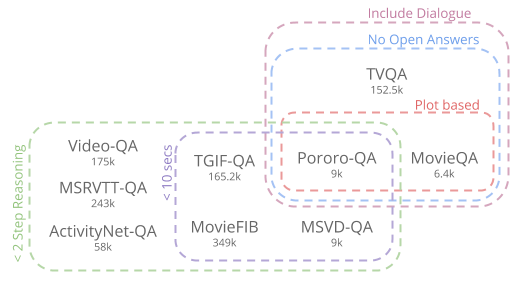
\includegraphics[width=0.8\linewidth]{Figures/figure_videoQA.png}
\end{center}
   \caption{The shortcomings of current VideoQA models.}
\label{fig:long}
\label{fig:onecol}
\end{figure}

%Expanding question-answering to videos has been gaining interest lately \mgm{passive voice and bad sentence}, and a small number of datasets have been produced. Some of these datasets incorporate both visual input and dialogue from a TV show or Movie \cite{}, and several of which ask plot-based, not exclusively vision based questions \cite{}. This is an important task, but since models based on these datasets tend to depend heavily on dialogue for long-term temporal reasoning \cite{}, our benchmark will focus on purely visual temporal reasoning. Of current benchmarks doing purely visual temporal reasoning, all but \cite{} refer to videos of less than 10 seconds long. Futhermore, all of them reason in simple (change wording) ways over time \cite{}. These are limited to x, y, z, frame based. MSRVTT-QA is also mostly 2 types of questions. Our dataset will be purely vision based, work on videos of 30-90 seconds long, and require a model to perform complex temporal reasoning. 

\subsection{Compositional Reasoning}

As questions become more complex, they often require of multiple reasoning steps in order to answer them. For example, the question "Was the person running or sitting for longer?" first requires finding the start and end of when the person was running and sitting, subtracting the start from the end, then comparing the lengths. A constrained set of logical steps (e.g. action localization, subtraction, comparison, etc) can be used as building blocks that are reordered to respond to a wide variety of different questions. This multi-step reasoning is called compositional reasoning because the overall understanding is composed of a series of smaller reasoning steps. Humans use compositional reasoning to learn quickly and generalize to novel combinations of ideas \cite{tani2014self, lake2018generalization, schulz2016probing}. 


\begin{figure}[t]
\begin{center}
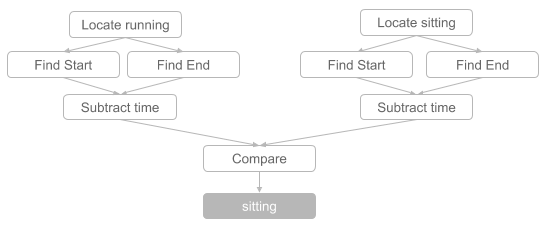
\includegraphics[width=0.8\linewidth]{Figures/figure_composition.png}
\end{center}
   \caption{The substeps required to answer the question "Was the person running or sitting for longer?".}
\label{fig:long}
\label{fig:onecol}
\end{figure}



Compositional questions have been used by ImageQA benchmarks to rigorously test models. Compositional questions tend to be longer, more complex, and use a wider variety of vocabulary. Furthermore, they can better test a model's reasoning ability by both requiring multiple steps of reasoning to answer the questions and by allowing for datasets to test generalizaton to novel compositions \cite{johnson2017clevr, hudson2019gqa, lake2018generalization}. For example, on the CLEVR dataset, the training questions could include the phrases "right of cube" and "behind sphere", but not "right of sphere" as a combination. Testing on this novel combination "right of sphere" in the test set tests a model's ability to generalize \cite{lake2018generalization, johnson2017clevr}. Many questions relevant to reasoning over videos require multi-step reasoning. A simple example covered by current datasets involves first localizing in time, then reasoning about that specific time. For example, this question from \cite{jang2017tgif}, "What does the bear on the right do after sitting?", requires finding when the bear stops sitting, then determining his activity after that. \mgm{Is this actually 3 b/c have to look at the bear?} Another way to reason compositionally is to refer to subjects indirectly, as the ImageQA benchmark \cite{hudson2019gqa} does with "What color is the food on the red object to the left of the girl?". 

Some ImageQA benchmarks use compositional reasoning extensively \cite{johnson2017clevr, hudson2019gqa}, but no VideoQA datasets go beyond two steps of compositional reasoning. Although these logical building block steps have been defined for ImageQA \cite{cheng2015break}, there are no compositional reasoning steps defined for temporal reasoning. Current models have struggled with multi-step reasoning, motivating a benchmark like ours that specifically explores compositional reasoning \cite{fan2019heterogeneous}.


\subsection{Scene Graphs}

Scene graphs are a symbolic representation of an image \cite{krishna2017visual}. The graph consists of nodes representing the objects in the image and edges representing relationships between these nodes. For each object node there are associated attributes. For example, an image with a man wearing white shorts would have an object node for "shorts" with "white" as an attribute and an object node for "man". These object nodes would be connected by an edge representing the relationship "wearing". Creating this symbolic representation of an image reduces it to its semantic parts. Using this representation has improved performance on many visual tasks such as visual question answering \cite{johnson2017inferring}, visual question answer generation \cite{hudson2019gqa}, relationship modeling \cite{krishna2018referring}, image captioning \cite{anderson2016spice}, image generation \cite{johnson2018image, ashual2019specifying}, and image retrieval \cite{ashual2019specifying, johnson2015image}.

Inspired by Visual Genome's scene graphs, \cite{ji2020action} annotated spatio-temporal scene graphs to create Action Genome. Spatio-temporal scene graphs consist of nodes representing objects and edges representing relationships between them \mgm{(add in that these relationships are 3 categories?)}. Each of these objects are associated with a specific frame in the video. The resulting effect is that a subject's relationships with the objects changes over time. Our project will use these spatial-temporal scene graphs to generate questions about videos. 

\section{Methods}

\subsection{Types of Temporal Reasoning}
To create our benchmark, we first established what types of temporal reasoning to explore. As mentioned previously, other vision-based datasets have looked exclusively at questions that could be answered with one frame, questions that refer to the entire video, and questions that ask "what happened" before, after, or while an event was occuring \cite{tapaswi2016movieqa, lei2018tvqa, jang2017tgif, kim2017deepstory, xu2017video, maharaj2017dataset, zeng2016leveraging, yu2019activitynet}. 

%\begin{itemize}
%	\item action sequencing
%	\item When actions precede, suceed, or coexist with one another
%	\item lengths of time activities occured
%	\item Reasoning about a subject's changing relationship with objects
%	\item Reasoning beyond action recognition after localizing within the video \mgm{does this make sense to normal people?}
%	\item comparative and logical operators 
%\end{itemize}

However, there are more types of temporal reasoning yet to be explored and tested on models. These new types include action sequencing, reasoning over the length of time activities occurred, reasoning with comparative and logical operators, and reasoning about when actions precede, succeed, or coexist with one another. Other questions could more deeply explore a subject's changing relationship with objects over time. 

%Finally, after localizing in time (e.g. before running), existing benchmarks do not require reasoning beyond action recognition, so other questions could require different types of 

% reasoning over a specified part of a video instead of just action recognition. \mgm{rewrite sentence} Since activities are composed of a subject's changing relationship with objects, questions can ask about those changes. Questions should also probe action sequencing and understanding ordering of actions within the video and when actions precede, succeed or coexist with one another. Current datasets do not ask questions about the lengths of time activities occurred. Beyond temporal reasoning, current VideoQA datasets do not do comparitive or logical (i.e. "and", "xor") questions. 
 
Our benchmark requires all the above types of reasoning to succeed. Future datasets may be able to expand even more by including sequences, bounding boxes, and time identifiers (e.g. she started running at 10.5 seconds) as answers.


\begin{figure}[t]
\begin{center}
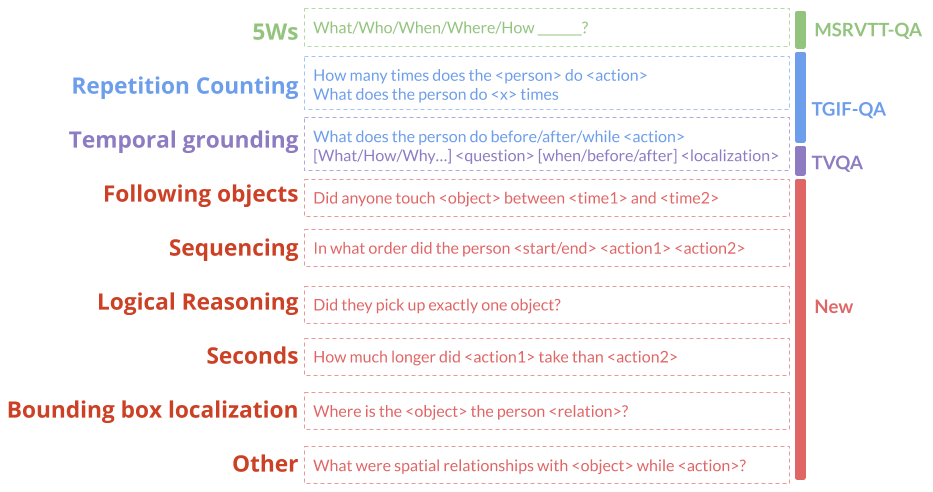
\includegraphics[width=0.8\linewidth]{Figures/figure_reasoning.png}
\end{center}
   \caption{Various types of temporal reasoning.}
\label{fig:long}
\label{fig:onecol}
\end{figure}


\subsection{Our Generation Pipeline}
Beyond exploring a wider variety of temporal concepts, an ideal benchmark would 1) be large, 2) mitigate biases in the answer distribution, 3) allow for novel compositions and 4) include a large suite of metrics. In order to achieve these goals, we automatically generate questions using a pipeline inspired by \cite{hudson2019gqa}.

The question generation pipeline consists of two parts: 1) augmenting spatio-temporal scene graphs to create detailed video representations and 2) building question templates with spaces for video-specific content. The first part of our pipeline uses dataset annotations from Action Genome and Charades \cite{ji2020action, sigurdsson2016hollywood} on Charades videos. These \mgm{30-90} second videos are filmed by non-professionals who act out everyday activities using 36 objects. Charades annotates the times actions occur, and Action Genome annotates attention, spatial, and contact relationships on a sample of frames. 

To make these scene graphs applicable for question answering, we first combine the annotations from both datasets into one data structure. We then created object and relationship nodes for action segmentation, adding in charades actions as a relationship category. We then supplement current annotations with their logical extensions. For example, if a person is carrying something, they are also holding it and touching it. With these adjustments, we have a filled out spatio-detailed spatio-temporal scene graph combining two datasets worth of annotations into a structure that can be fed into the question templates. An important limitation to note is that although these scene graphs are detailed, our questions depend on their annotations, so any errors in those datasets affects ours.
    
The second part of our pipeline consists of question templates that each have a natural language sentence with tags representing different elements categories in the video, such as in the question "What were they $<$contact relationship$>$?". Each template also contains information about the question's structural and semantic contents. 

To generate a question-answer pair, our system combines a spatio-temporal scene graph with these templates by replacing the tags with elements of the corresponding types. For a video where the person is holding a blanket while sitting on a chair, our pipeline would create both questions "What were they holding?" and "What were they sitting on?". Given the scene graph information, we then automatically determine the answers "blanket" and "chair" respectively. 

These tags can be filled with both direct and indirect references. For example, an $<$object$>$ tag's direct reference would be "blanket" but an indirect reference would be "the object they were holding". We ensure that there are no questions that give away the answers (e.g. "Were they holding the object they were holding?"). Indirect references can also be recursive. The object tag listed above could also be replaced with "the object they were holding after closing the door" or "the object they were holding after the shortest action". Indirect references require locating the referred object, action, relationship, or time in video before reasoning about the question as a whole, leading to complex questions that require multiple reasoning steps. 

\begin{figure}[t]
\begin{center}
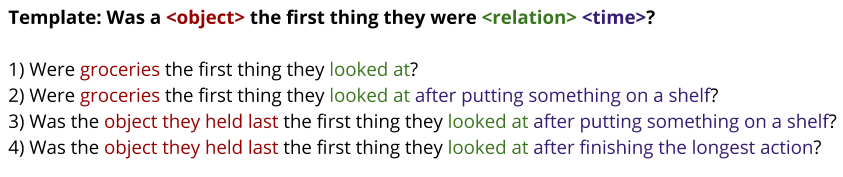
\includegraphics[width=0.8\linewidth]{Figures/figure_indirect.png}
\end{center}
   \caption{Various types of temporal reasoning.}
\label{fig:long}
\label{fig:onecol}
\end{figure}



This procedure to generate questions allows us to work towards the qualities of an ideal benchmark.
    
\subsection{Is large}
    
    Human annotation of question-answer pairs for video is time consuming and expensive. Automatically generating questions allows us to create a much larger dataset of \mgm{add here}. Automatically generated datasets have previously been criticized for lacking diversity \cite{yu2019activitynet}. We have \mgm{add} templates asking a wide variety of questions. Each template is also associated with multiple natural language versions of the same question. Indirect reference tags expand complexity even further.
    
    \mgm{make some sort of graphic comparing size?}

\subsection{Mitigates biases in answer distribution}
    
    Many ImageQA benchmarks do not accurately determine a model's reasoning ability because skews in their answer distributions reduce dependence on visual input and increase reliance on the relative prevalence of different answers in the data \cite{hudson2019gqa, goyal2017making}. Although there has not been an in depth analysis of skewed answer distributions in Video QA biases, our dataset, if left unbalanced, would be skewed. For example, a person is covered by a blanket 6721 times but standing on a blanket only 32 times. Consequently, the answer to the question "What were they doing to the blanket?" is much more likely to be "covered by" rather than "standing on". To avoid inflated accuracy scores, we want to retain the same distribution (i.e. still have more instances where the answer is "covered by"), but smooth the answer distribution to make the differences less extreme. We balance the answer distribution for each category using the same process as \cite{hudson2019gqa} to downsample highly popular answers to shift probability into the tail of the distribution. \mgm{Talk about the process in detail for doing that? Global vs local variables}. \mgm{Include graphs}. Our question generation pipeline allows for this balancing because we have the structural and semantic information associated with each template to split the questions into relevant categories before balancing. 
    
    \begin{figure}[t]
\begin{center}
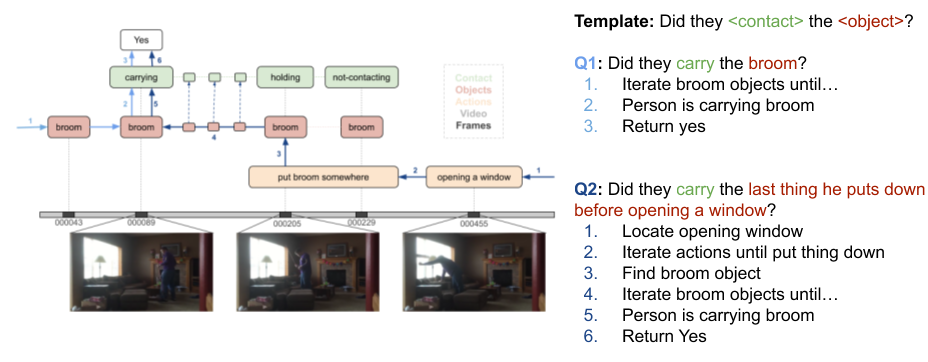
\includegraphics[width=0.8\linewidth]{Figures/figure_compareQs.png}
\end{center}
   \caption{Various types of temporal reasoning.}
\label{fig:long}
\label{fig:onecol}
\end{figure}

    
   \subsection{Tests novel composition}
    
    An important part of human reasoning is the ability to generalize concepts of the same category to novel compositions. For example, in the training set the model may see the phrases "before running" and "the action they did the longest". Then, in the test set, we can test if they understand the idea of "before the action they did the longest". We are able to create such a training and testing split to judge these novel compositions because we have knowledge of what temporal localization, logical reasoning, and indirect tags are in each question. \mgm{Potentially VG slide 18 for how to solve them?}
    


    \subsection{Has a suite of new metrics}
    
    Finally, we want to be able to complexly analyze a model's various abilities across different types of temporal and logical reasoning. We can achieve better measurements by choosing different types of questions from the training and test sets based on qualities of the questions. We are able to do this because our pipeline gives us control over the content of all the questions. We have not accomplished this step thus far in the 10 weeks of the DREU program, however we plan to incorporate it by the end of the summer. 

\section{Results}

A the end of the 10 weeks of DREU, we have completed \mgm{this many} templates and generated them for 500 videos, creating \mgm{this many} question-answer pairs. Our final Video QA dataset consists of three parts: the Charades videos, without any annotations or the corresponding spatio-temporal scene graphs. the questions, the answers. 

In other words, Our Benchmark = $\{ V, Q, A \}$, where every $v_i \in V$ corresponds to a list of questions $q_i  \in Q$ and a list of corresponding answers $a_i \in A$. For every question $q_ij \in q_i$ there is a corresponding answer $a_ij \in q_i$. Each $q_ij$ is associated with binary flags determining if it is included in each metric.



Break down the dataset into better stats.  By global and local? or by action? by steps?

Pre and post balancing



Do things like average length of question vs average length of other questions in other datasets

Example questions? Maybe as a figure




\section{Future work}

To complete this project, we plan to expand upon our current progress in three ways. First, we will create a wider variety of templates, both in the subject of what they ask and in the natural language question. Second, we will develop a suite of metrics. Third, we will evaluate existing VideoQA models on our dataset \cite{le2020hierarchical, fan2019heterogeneous, li2019beyond}

We want our benchmark to be able to provide a complex analysis of the abilities of VideoQA models. Therefore, we will create a suite of metrics, each of which measures a different aspect of performance, as specified in Table \mgm{how to refer to this?}. Content Category metrics ask how well the model performs overall and on different question and answer categories. Generalization metrics ask if given a small portion of basic concepts, can the model generalize to more complex questions. Answer legitimacy metrics ask if the model has a consistent and plausible understanding of the contents of the video. Our suite of metrics will provide insight on these questions and a more detailed understanding of the model's strengths and weaknesses.



\begin{table}[]
    \begin{center}
    \caption{Suite of Metrics}
    \label{tab:table1}
    \begin{tabular}{|p{2cm}|p{5cm}|}
     \hline
     \multicolumn{2}{|c|}{\textbf{Content Category}}\\
    \hline
    All & Accuracy on all questions\\
    \hline
    Question Type & Accuracy on each question category (e.g. Counting, Length, First, ...)\\
    \hline
    Answer Type & Accuracy on each answer category (e.g. binary, and open)\\
    \hline
    
    
     \multicolumn{2}{|c|}{\textbf{Generalization}}\\
    \hline
    Video length & train on videos of length $<$ 30 seconds. Test on videos of length $\geq$ 30 seconds \\
    \hline
    Actions & train on videos with $<$ 5 actions. Test on videos with $\geq$ 5 actions  \\
    \hline
    Compositional Steps &  train on questions with $<$ 6 steps. Test on questions with $\geq$ 6 steps  \\
    \hline
    Novel Compositions & TODO \\
    \hline
    Indirect ref Consistency & TODO \\
    \hline
    \% training data & train on only 1, 5, 10 and 20 percent of training data \\
    \hline
    
    
     \multicolumn{2}{|c|}{\textbf{Answer Legitimacy}}\\
    \hline
    TODO & Something where sequencing is consistent \\
    \hline
    Consistent & If answers a question correctly, answers all logical entailments correctly \\
    \hline
    Validity & Answer type is of correct genre (e.g. object, relation, action, count, yes/no)\\
    \hline
    Plausibility  & Answer exists in distribution for that question\\
    \hline
    Distribution & Predicted answers follow same distribution as ground truth\\
    \hline
    \end{tabular}
    \end{center}
\end{table}

\section{Conclusion}
Our project contributes a dataset of question-answer pairs for video, a pipeline for creating question answer pairs from spatio-temporal scene graphs, and a suite of metrics on which to measure performance.
Our benchmark will facilitate the creation of VideoQA models by providing a challenging task.

{\small
\bibliographystyle{ieee_fullname}
\bibliography{dreu_final}
}

\end{document}
